% \documentclass{acmart}
\documentclass{article}
\usepackage{graphicx}
\usepackage[utf8]{inputenc}
\usepackage[T1]{fontenc}
\usepackage{pgfplots}
\usepackage{pgfplotstable} 
\usepackage{titlesec}
\usepackage{lipsum}
\usepackage{authblk}
\usepackage{amsmath}
\usepackage{algorithm}
\usepackage{amsmath}
\usepackage[noend]{algpseudocode}
\usepackage {tikz}
\usetikzlibrary {positioning}
\algrenewcomment[1]{\(\triangleright\) #1}
\algnewcommand{\LineComment}[1]{\State \(\triangleright\) #1}

\titleformat{\chapter}[display]{\normalfont\bfseries}{}{0pt}{\Large}

\begin{document}

\title{Cobertura exata por conjuntos: modelagem alternativa do problema das N rainhas}
\author{João Mateus de Freitas Veneroso}
\affil{Departamento de Ciência da Computação da Universidade Federal de Minas Gerais}

\maketitle

\section{Introdução}

Este artigo discute o problema NP-completo de cobertura exata de conjuntos e, em particular,
a solução para o problema das N rainhas por meio de três abordagens diferentes: 
o algoritmo de backtracking de Dijkstra \cite{djikstra1972}, o algoritmo Dancing Links (DLX) de Knuth e o algoritmo
DLX com a utilização da heurística S \cite{knuth2000}. Embora o algoritmo Dancing Links também seja baseado no paradigma
backtracking, ele utiliza uma estrutura de dados otimizada que reduz significativamente 
o tempo de execução. Além disso, a heurística S é uma estratégia de poda que visa reduzir o número de 
subproblemas, reduzindo o espaço de busca por soluções. Este artigo vai investigar e comparar as
estratégias listadas em termos do número de subproblemas e do tempo de execução.

\section{Cobertura exata de conjuntos}

O problema de cobertura exata por conjuntos pode ser descrito da seguinte forma: 
dada uma coleção $ S $ de subconjuntos de um conjunto $ C $, $ S^* \subseteq S $ é uma cobertura exata de C se 
todo subconjunto $S_i \in S^*$ é disjunto em relação aos demais subconjuntos de $ S^* $ e $ S_1 \cup S_2 \cup ... \cup S_n = C $. Ou
seja, todo elemento $ x \in C $ deve aparecer em um único subconjunto de $ S^* $. O problema da 
cobertura exata é o problema número 14 dos 21 problemas NP-completos descritos por Karp em 1972 \cite{karp1972}.

Perceba que o problema de cobertura exata de conjuntos é um caso particular do problema de cobertura de conjuntos, também
NP-completo. No problema de cobertura de conjuntos não existe a necessidade dos subconjuntos da solução serem disjuntos.
Portanto, dado um conjunto $ \mathcal{S} = \{ A, B, C, D, E \} $ e subconjuntos $ \mathcal{X} = \{ A, B, C \} $ e 
$ \mathcal{Y} = \{ C, D, E \} $, a subcoleção
$ \{ \mathcal{X}, \mathcal{Y} \} $ representa uma solução para o problema de cobertura de conjuntos, porém não representa uma solução válida para 
o problema de cobertura exata. A limitação adicional no problema de cobertura exata torna muito difícil encontrar 
algoritmos que encontrem soluções aproximadas para o problema, uma vez que se torna complicado até mesmo definir o que 
seria uma solução aproximada. Por conta disto, o que nos resta é pensar em estratégias inteligentes
de backtracking que reduzam o espaço de busca. Estas estratégias serão exploradas nas próximas seções.

\subsection{Representação em grafo}

\begin{figure}
  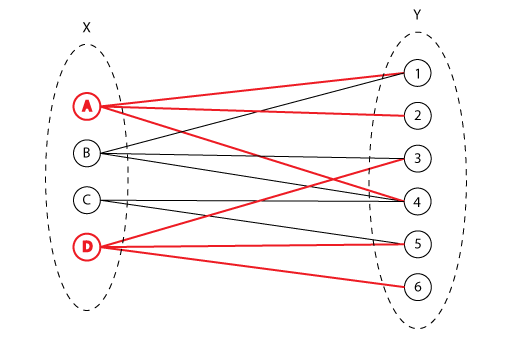
\includegraphics[width=\linewidth]{graph.png}
  \caption{Exemplo de representação em grafo de uma cobertura exata}
  \label{fig:graph}
\end{figure}

O problema de cobertura exata de conjuntos pode ser representado por um grafo não direcionado bipartido onde os vértices são
divididos em dois conjuntos disjuntos $ X $ e $ Y $. Dado um conjunto $ \mathcal{S} $ para o qual se procura uma cobertura exata,
o conjunto $ X $ contém os subconjuntos de $ \mathcal{S} $ e o conjunto $ Y $ contém
os elementos de $ \mathcal{S} $. Se um subconjunto de $ X $ contiver um elemento de $ Y $ haverá uma aresta no grafo ligando o subconjunto
ao elemento. A figura \ref{fig:graph} apresenta um exemplo de cobertura exata em grafos no qual $ \mathcal{S} = \{ 1, 2, 3, 4, 5, 6 \} $
e os subconjuntos de $ \mathcal{S} $ são:

\begin{itemize}
\item $ A = \{ 1, 2, 4 \} $
\item $ B = \{ 1, 3, 4 \} $
\item $ C = \{ 4, 5 \} $
\item $ D = \{ 3, 5, 6 \} $
\end{itemize}

Nesse caso, $ A $ e $ D $ são disjuntos e $ A \cup B = \mathcal{S} $. Portanto, $ \{ A, D \} $ é uma cobertura exata de $ \mathcal{S} $.

\subsection{Representação em matriz} \label{sec:matrixrepresentation}

Uma modelagem alternativa do problema de cobertura exata se dá por meio da utilização 
de uma matriz booleana onde as colunas representam elementos e as linhas representam subconjuntos. Para o exemplo
descrito na figura \ref{fig:graph}, construiríamos a matriz equivalente:

\[
\begin{bmatrix}
    1 & 1 & 0 & 1 & 0 & 0 \\
    1 & 0 & 1 & 1 & 0 & 0 \\
    0 & 0 & 0 & 1 & 1 & 0 \\
    0 & 0 & 1 & 0 & 1 & 1
\end{bmatrix}
\]

Nesse caso, o problema se torna encontrar conjuntos de linhas que contenham exatamente um 1 em cada coluna. Para
o exemplo em questão a única solução se dá pelas linhas 1 e 4, que representam os subconjuntos A e D, respectivamente.
Esta abordagem para o problema de cobertura exata é muito útil no contexto do algoritmo DLX.

\subsection{Exemplos concretos do problema}

Alguns exemplos concretos do problema de cobertura exata de conjuntos são o quebra-cabeça Sudoku,
o problema de Polyomino tiling, o problema de construção de quadrados latinos e o problema das
N-rainhas, que será explorado nas próximas seções.

\section{N-rainhas}

O problema das N-rainhas ou N-damas consiste em dispor N rainhas em um tabuleiro de xadrez com $N \times N$ casas para qualquer
$ N \geq 4 $ de forma que nenhuma rainha seja atacada por outra. Portanto, nenhuma rainha pode ocupar a mesma linha, coluna ou diagonal
do tabuleiro. O caso clássico se dá para $ N = 8 $, mas aqui exploraremos como os algoritmos se comportam com diversos valores de N. 

\subsection{Solução de Dijkstra para o problema das N-rainhas}

Se tivéssemos de testar todas as combinações com N rainhas no tabuleiro, o número de possibilidades seria
tão grande que tornaria a solução do problema impraticável. Tomando o problema das 8 rainhas por exemplo,
o número de combinações seria $ 64!/56! $ ou aproximadamente $ 2^{47} $. A solução de Djikstra \cite{dijkstra1972} utiliza
cinco propriedades do problema para reduzir o número de combinações a um número praticável. 
As propriedades são:

\begin{itemize}
\item Toda linha deve conter precisamente uma rainha
\item Toda coluna deve conter precisamente uma rainha
\item Existem 2N - 1 diagonais no sentido da diagonal principal, das quais N contém uma rainha
\item Existem 2N - 1 diagonais no sentido da diagonal secundária, das quais N contém uma rainha
\item Dada uma configuração onde nenhuma rainha seja atacada por outra, a remoção de uma das rainhas preserva esta propriedade
\end{itemize}

Tendo em vista as propriedades descritas, podemos construir um algoritmo de backtracking eficiente para encontrar todas as
soluções do problema. Para guardar quais posições do tabuleiro estão livres poderíamos utilizar uma representação em matriz
$ N \times N $, no entanto, cada atualização poderia ter de alterar o valor de até $ 3N - 1 $ quadrados. Portanto, utilizaremos
uma representação otimizada com três arranjos representando as colunas ocupadas, as diagonais primárias ocupadas e as diagonais 
secundárias ocupadas. Dessa forma, apenas três valores terão de ser alterados para cada rainha posicionada. Além disso, é útil 
lembrar que todos os quadrados em uma diagonal primária tem a mesma diferença de índices de linha e coluna. E todos os quadrados 
em diagonais secundárias tem a mesma soma entre os índices de linhas e das colunas. Dessa forma, podemos indexar o 
arranjo das diagonais por meio destas somas e diferenças para acelerar a atualização da estrutura. No problema das 8 rainhas
por exemplo, teríamos a seguinte estrutura de arranjos booleanos:

\begin{itemize}
\item Colunas: cols[0:7]
\item Diagonais principais: up[-7:7]
\item Diagonais secundárias: down[0:14]
\end{itemize}

Logo, para verificar se uma posição (i,j) do tabuleiro está livre basta checar os três arranjos com a seguinte expressão: \\

col[j] and up[i - j] and down[i + j] \\

\begin{algorithm}
\begin{algorithmic}[1]
\State {integer $ N $; }
\State {integer array $ x[0:N-1] $; }
\State {boolean array $ col[0:N-1] $; }
\State {boolean array $ up[-(N-1):(N-1)] $; }
\State {boolean array $ down[0:2N - 2] $; }

\Procedure{BacktrackingNQueensAux}{n}
  \If {$ n = N $}
    \State {Imprime Solução}
    \Return
  \EndIf

  \For{ $ h = 1 $; $ h \leq N $; $ h \gets h + 1 $ } 
    \If {$ col[h] $ \textbf{and} $ up[n - h] $ \textbf{and} $ down[n + h] $}
      \State {$ x[n] \gets h $;}
      \State {$ col[h] \gets false $; $ up[n - h] \gets false $; $ down[n + h] \gets false $;}
      \State $ BacktrackingNQueensAux(n + 1) $
      \State {$ col[h] \gets true $; $ up[n - h] \gets true $; $ down[n + h] \gets true $; }
    \EndIf
  \EndFor
\EndProcedure

\Procedure{BacktrackingNQueens}{N}
  \For{ $ k = 1 $; $ k \leq N $; $ k \gets k + 1 $ } 
    \State {$ col[k] \gets true $}
  \EndFor
  \For{ $ k = 1 $; $ k \leq 2N - 1 $; $ k \gets k + 1 $ } 
    \State {$ up[k - N + 1] \gets true $}
    \State {$ down[k] \gets true $}
  \EndFor

  \State {BacktrackingNQueensAux(1)}
\EndProcedure

\end{algorithmic}
\caption{Backtracking N-queens}\label{alg:alg_1}
\end{algorithm}

Adicionalmente, é necessário manter um arranjo de inteiros com N elementos que guardará
os índices das rainhas em cada linha e servirá de estrutura base para a iteração. 
Ao colocar a rainha número N no tabuleiro sabemos que chegamos a uma solução válida e
podemos imprimir a posição de cada uma das rainhas pelo índice da sua linha.
O pseudocódigo está descrito no algoritmo \ref{alg:alg_1}. 

\subsection{Algoritmo DLX}

O algoritmo X implementado em termos de Dancing Links (DLX) descrito por Knuth \cite{knuth2000} 
encontra todas as soluções para um problema de cobertura exata representado no formato de
uma matriz de 0s e 1s, conforme descrito na seção \ref{sec:matrixrepresentation}. No caso
do problema das N-rainhas, podemos modelar a solução com base em uma matriz onde as linhas correspondem
aos $ N^2 $ diferentes quadrados do tabuleiro de xadrez e as colunas correspondem à quatro grupos:

\begin{itemize}
\item N colunas correspondentes às linhas do tabuleiro de xadrez
\item N colunas correspondentes às colunas do tabuleiro de xadrez
\item 2N - 3 colunas correspondentes às diagonais principais do tabuleiro de xadrez
\item 2N - 3 colunas correspondentes às diagonais secundárias do tabuleiro de xadrez
\end{itemize}

\begin{center}
  \begin{table}
  \centering
  \begin{tabular}{ c c c c }
    i & j & Up & Down  \\
    0 & 0 & 0   & 0    \\
    0 & 1 & -1  & 1    \\
    0 & 2 & -2  & 2    \\
    0 & 3 & -3  & 3    \\
    1 & 0 & 1   & 1    \\
    1 & 1 & 0   & 2    \\
    1 & 2 & -1  & 3    \\
    1 & 3 & -2  & 4    \\
    2 & 0 & 2   & 2    \\
    2 & 1 & 1   & 3    \\
    2 & 2 & 0   & 4    \\
    2 & 3 & -1  & 5    \\
    3 & 0 & 3   & 3    \\
    3 & 1 & 2   & 4    \\
    3 & 2 & 1   & 5    \\
    3 & 3 & 0   & 6    \\
  \end{tabular}
  \caption{Problema das 4 rainhas na forma de matriz}
  \label{tab:matrix_3_queens}
  \end{table}
\end{center}

A tarefa do algoritmo se torna encontrar uma cobertura exata para as colunas correspondentes às
linhas e colunas do tabuleiro de xadrez, enquanto utilizamos no máximo uma vez cada elemento das
colunas correspondentes às diagonais do tabuleiro. Perceba que o número de colunas para as diagonais
é $ 2N - 3 $ e não $ 2N - 1 $ como seria esperado. Isso acontece pois os quadrados dos cantos
superior esquerdo e inferior direito são os únicos por onde passam as suas diagonais secundárias e 
os quadrados dos cantos superior direito e inferior esquerdo são os únicos por onde passam suas diagonais
principais, portanto não há possibilidade de existir conflito nestas diagonais e se torna desnecessário incluir as colunas 
correspondentes na matriz. Um exemplo de matriz para o problema das 4 rainhas se dá pela tabela \ref{tab:matrix_3_queens}. No
caso desta tabela, ao invés de incluir todas as colunas da matriz foi incluído apenas o índice da coluna
referente ao seu grupo com a notação utilizada no algoritmo de Backtracking de Dijkstra. Note que uma solução possível para o 
problema é o conjunto de linhas { 1, 8, 10, 15 } que cobre todos os valores dos índices i e j sem repetir os valores das
colunas Up e Down.

O algoritmo DLX consiste basicamente em construir a matriz descrita acima por meio de listas duplamente encadeadas.
As linhas da matriz são listas onde cada elemento está conectado por ponteiros aos elementos à sua esquerda e à sua direita de forma 
toroidal, ou seja, o último elemento da linha está conectado ao primeiro pelo seu ponteiro direito e o primeiro elemento está conectado
ao último pelo seu ponteiro esquerdo. Da mesma forma, as colunas tem o mesmo tipo de ligação, onde cada elemento está conectado aos elementos
superior e inferior de forma toroidal. Além disso, cada coluna possui uma lista de cabeçalho, aos quais todos os elementos da coluna
estão conectados. Cabe ressaltar neste momento que, no caso das N-rainhas por exemplo, apenas as colunas primárias referentes 
aos índices das linhas e das colunas do tabuleiro estarão ligadas entre si. Os ponteiros L e R das colunas secundárias referentes às diagonais 
serão nulos. O motivo disso ficará aparente no pseudo código do algoritmo.

Cada elemento x = 1 da matriz pode ser representado por um objeto com os seguintes campos: U[x], D[x], L[x], R[x], C[x], onde
U aponta para o elemento de cima, D aponta para o elemento de baixo, L aponta para o elemento da esquerda, R aponta para o elemento da direita e
C aponta para o cabeçalho da coluna. Além dos campos descritos, o cabeçalho possui os campos size, que indicam o número de 1s na coluna, 
e o campo name, que indica o nome da coluna. Por fim, existe um objeto root que simplesmente aponta para o primeiro item do cabeçalho.

A cada iteração do algoritmo, escolhemos uma coluna da matriz e, para cada linha naquela coluna (lembrando que a nossa lista encadeada
só contém as linhas cujo valor naquela coluna é 1),
adicionamos aquela linha à resposta e retiramos da matriz todas as linhas e colunas conflitantes. Em posse 
da nova matriz diminuída repetimos o processo até que tenhamos coberto todas as colunas encontrando uma resposta válida
ou descobrindo que não há resposta naquele ramo da árvore de busca se ainda houverem colunas descobertas e não existirem 
mais linhas na matriz. Fazemos então o processo de backtracking recolocando as linhas e colunas conflitantes na matriz e 
repetindo o processo para a próxima linha.

O processo de remoção e reinserção de colunas na matriz é muito eficiente porque os ponteiros dos elementos removidos 
nunca são apagados. Por exemplo, digamos que o elemento x foi removido. Para reinserí-lo na sua antiga linha basta 
realizar a operação: \\

R[L[x]] = x e L[R[x]] = x \\

A operação de reinserção na coluna é análoga. 


\begin{algorithm}
\begin{algorithmic}[1]
\State{Object Array Root} \Comment{Guarda a representação em listas encadeadas da matriz}
\State{Object Array O} \Comment{Arranjo de linhas que constituem uma solução}

\Procedure{ImprimirSolução}{}
  \For{$ O_k \in O $} 
    \For{i := R[$O_k$], i := R[R[$O_k$]] ...} 
      \State{Print Name[C[i]]}
    \EndFor
  \EndFor
\EndProcedure

\Procedure{RemoverColuna}{col}
  \State{L[R[col]] := L[col]}
  \State{R[L[col]] := R[col]}

  \For{i := D[col], i := D[D[col]] ...} 
    \For{j := R[i], j := R[R[i]] ...} 
      \State{U[D[j]] := U[j]}
      \State{D[U[j]] := D[j]}
      \State{Size[C[j]] := Size[C[j]] - 1}
    \EndFor
  \EndFor
\EndProcedure

\Procedure{ReinserirColuna}{col}
  \For{i := U[col], i := U[U[col]] ...} 
    \For{j := L[i], j := L[L[i]] ...} 
      \State{U[D[j]] := j}
      \State{D[U[j]] := j}
      \State{Size[C[j]] := Size[C[j]] + 1}
    \EndFor
  \EndFor

  \State{L[R[col]] := col}
  \State{R[L[col]] := col}
\EndProcedure

\Procedure{DlxNQueensAux}{k}
  \If {R[Root] = Root}
    \State {ImprimirSolução()}
    \Return
  \EndIf
  
  \State {col := EscolherColuna() }
  \State {RemoverColuna(col) }
  
  \For{linha := D[col], linha := D[D[col]] ...} 
    \State{$ O_k $ := linha}
    \For{el := R[linha], el := R[R[linha]] ... } 
      \State{RemoverColuna(el)}
    \EndFor

    \State{DLXNQueensAux(k + 1)}

    \For{el := L[linha], el := L[L[linha]] ... } 
      \State{ReinserirColuna(el)}
    \EndFor
  \EndFor
  \State{ReinserirColuna(col)}
\EndProcedure

\Procedure{DLXNQueens}{N}
  \State{InicializarMatriz() }
  \State{DLXNQueenAux(0) }
\EndProcedure

\end{algorithmic}
\caption{DLX N-queens}\label{alg:alg_2}
\end{algorithm}

O pseudocódigo do algoritmo DLX para o problema das N-rainhas está descrito no algoritmo \ref{alg:alg_2}.
O procedimento InicializarMatriz cria as listas encadeadas correspondentes à matriz para o problema das N-rainhas
e inicializa o elemento Root. As soluções para o problema constituem em conjuntos de linhas que façam uma cobertura
exata da matriz. A variável O guarda as linhas à medida que o algoritmo progride e a função ImprimirSolução imprime
o identificador das colunas destas linhas. A função EscolherColuna, a princípio pode escolher sempre a primeira coluna 
da matriz, mas na próxima seção, exploraremos estratégias de escolha mais inteligentes. Por último, o atributo Size do 
cabeçalho parece não fazer nada no algoritmo descrito. No entanto, a sua importância ficará clara
na próxima seção, que explora uma heurística para ampliar a eficácia do algoritmo DLX.

\subsection{Heurística S}

A heurística S consiste em uma estratégia inteligente de escolha das colunas no algoritmo DLX. Knuth
observou que ao escolhermos a coluna que contém o menor número de 1s estaremos minimizando o
número de subproblemas a serem resolvidos, uma vez que, para cada 1 na coluna, um novo galho da árvore de subproblemas é gerado.
A implementação desta heurística é muito simples levando em conta que no algoritmo \ref{alg:alg_2} já salvamos no 
cabeçalho o número de 1s de cada coluna. Portanto, basta que a função EscolherColuna retorne a coluna com o menor
atributo Size.

Além da heurística S, utilizaremos uma outra heurística para acelerar a solução do problema das N-rainhas.
É melhor colocar as rainhas nas casas do meio do tabuleiro antes das extremidades, pois estas casas
normalmente limitam mais a colocação das próximas rainhas, diminuindo a quantidade de subproblemas.
Por exemplo, considerando o problema das 4 rainhas, a ordem de prioridade para colocação das peças nas 
linhas (L1, L2, L3, L4) e colunas (C1, C2, C3, C4) seria: L3, C3, L2, C2, L4, C4, L1, C1. Dessa forma,
caso duas colunas possuam o mesmo Size pela heurística S, o desempate será feito por meio desta ordem de prioridade.

A próxima seção apresenta resultados experimentais para a resolução do problema das N-rainhas utilizando cada um dos algoritmos
e heurísticas apresentados até agora.

\section{Experimentos}

Os experimentos testaram o desempenho de 3 algoritmos para o problema das N-rainhas: Backtracking N-Queens,
DLX e DLX com a heurística S. O número de rainhas variou entre 4 e 20 e foi medido o tempo de execução
e o número de nodos da árvore de subproblemas em cada caso. O resultado dos experimentos está descrito na tabela
\ref{tab:tab_2}. Todos os algoritmos foram implementados em Python.

\begin{center}
  \begin{table}
  \centering
  \begin{tabular}{ c c c c }
    Rainhas & Número de Soluções & Tempo BT & Tempo DLX & Tempo DLX+S & Nodos BT & Nodos DLX & Nodos DLX+S \\
    4       & 0 & 0   & 0    \\
    5       & 1 & -1  & 1    \\
    6       & 2 & -2  & 2    \\
    7       & 3 & -3  & 3    \\
    8       & 0 & 1   & 1    \\
    9       & 1 & 0   & 2    \\
    10       & 2 & -1  & 3    \\
    11       & 3 & -2  & 4    \\
    12       & 0 & 2   & 2    \\
    13       & 1 & 1   & 3    \\
    14       & 2 & 0   & 4    \\
    15       & 3 & -1  & 5    \\
    16       & 0 & 3   & 3    \\
    17       & 1 & 2   & 4    \\
    18       & 2 & 1   & 5    \\
    19       & 3 & 0   & 6    \\
    20       & 3 & 0   & 6    \\
  \end{tabular}
  \caption{Resultados dos experimentos}
  \label{tab:tab_2}
  \end{table}
\end{center}

\bibliography{bibliography} 
\bibliographystyle{ieeetr}

\end{document}
